\documentclass{article}

\usepackage[margin=1in]{geometry}
\usepackage{amsmath}
\usepackage{amsfonts}
\usepackage{graphicx}
\usepackage{float}
\usepackage{caption}
\usepackage{color}
\usepackage{listings}

\definecolor{mygreen}{RGB}{28,172,0}
\definecolor{mylilas}{RGB}{170,55,241}

\title{Homework 4: Digital Control (ECEN 5458)}
\author{Zachary Vogel}
\date{\today}

\newcommand{\rank}{\text{rank}}

\begin{document}

\lstset{language=Matlab,%
    %basicstyle=\color{red},
    breaklines=true,%
    morekeywords={matlab2tikz},
    keywordstyle=\color{blue},%
    morekeywords=[2]{1}, keywordstyle=[2]{\color{black}},
    identifierstyle=\color{black},%
    stringstyle=\color{mylilas},
    commentstyle=\color{mygreen},%
    showstringspaces=false,%without this there will be a symbol in the places where there is a space
    numbers=left,%
    numberstyle={\tiny \color{black}},% size of the numbers
    numbersep=9pt, % this defines how far the numbers are from the text
    emph=[1]{for,end,break},emphstyle=[1]\color{red}, %some words to emphasise
    %emph=[2]{word1,word2}, emphstyle=[2]{style},    
}
\maketitle

\section*{Problem 1}
Problem 7.2 from the book.\\
A servomechanism system is expected to have a rise time of no more than 10 milliseconds and an overshoot of no more than 5\%. Solve the following problems.
\subsection*{(a)}
Plot in the s-plane the corresponding region of acceptable closed-loop pole locations.\\

Given that $\omega_n\geq \frac{1.8}{t_r}=180$, and $\zeta\approx 0.6(1-M_p)=0.57$ we can draw the diagram.
\begin{figure}[H]
    \centering
    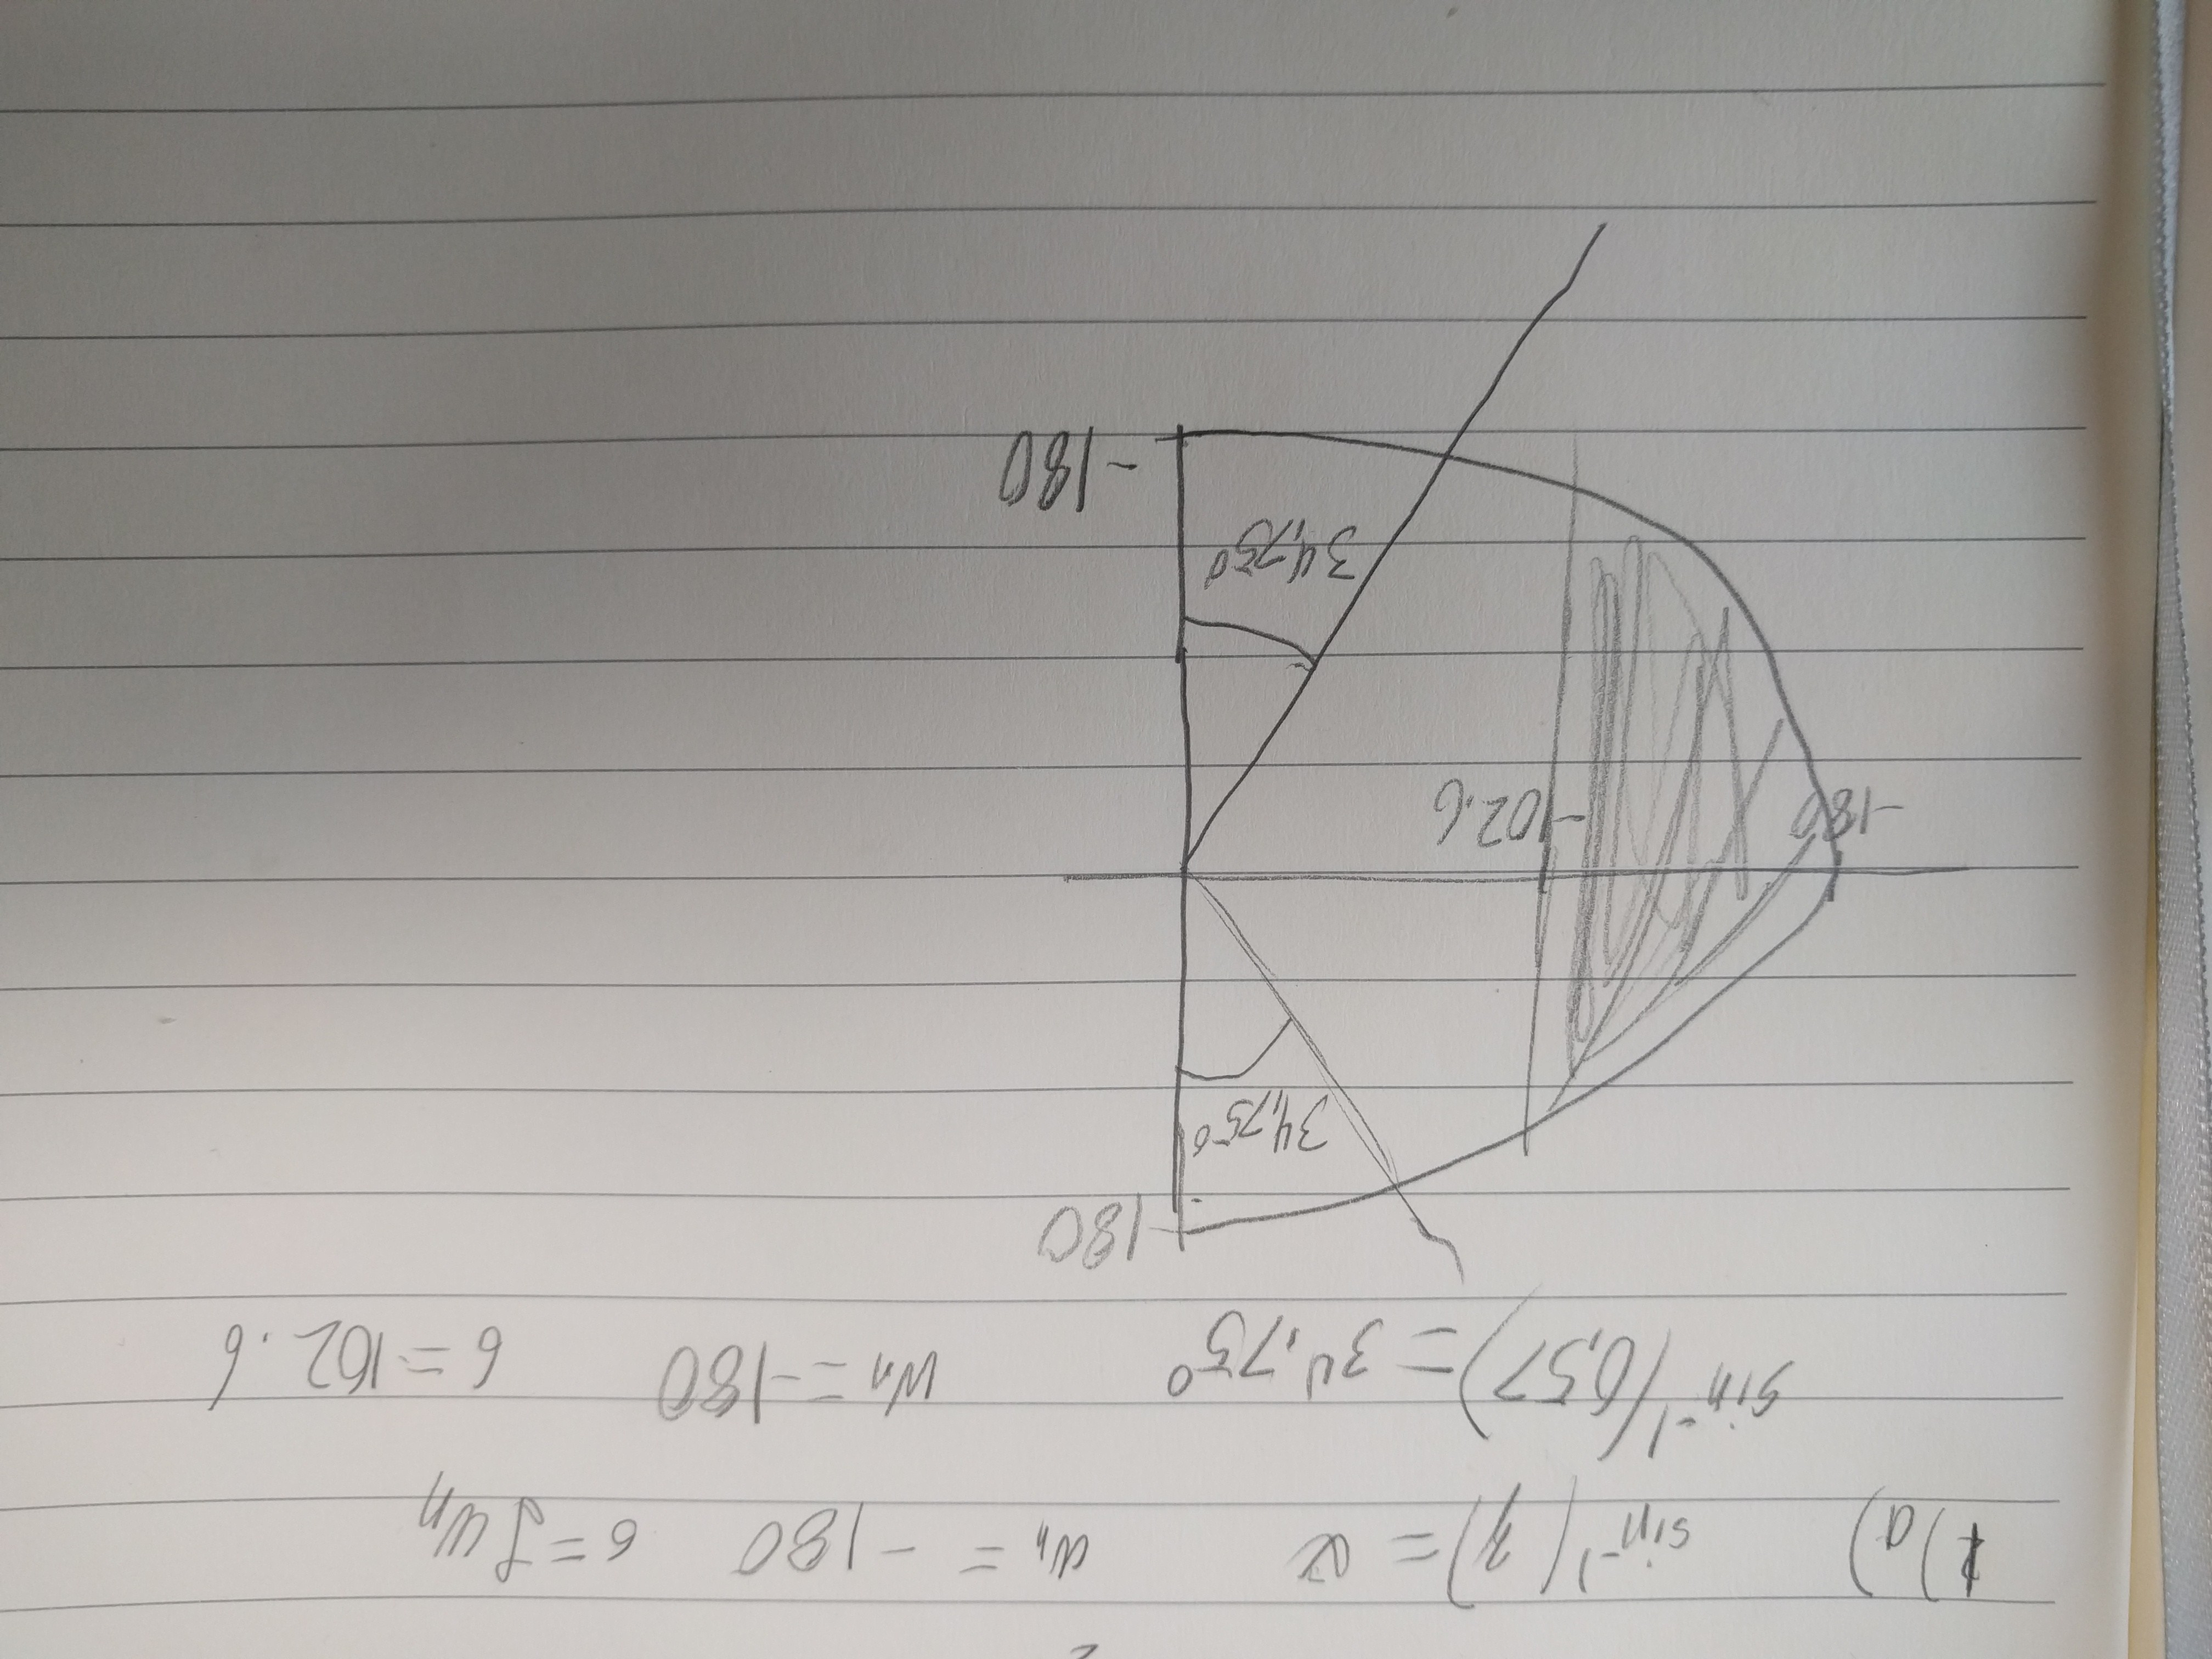
\includegraphics[width=0.7\textwidth,angle=180]{PR1_region.jpg}
    \caption{The region where the poles need to be to meet the constraints of the system}
\end{figure}
\subsection*{(b)}
What is the estimated Bode gain corssover frequency (rad/sec)?\\

Since $\omega_n\approx\omega_c$ the crossover frequency is about 180 radians per second.

\subsection*{(c)}
What is the estimated phase margin in degrees?\\

Since $PM\approx 100*\zeta$ the phase margin is about $57^\circ$.

\subsection*{(d)}
What is the sample period, T, if the estimated phase shift due to the sample and hold is to be no more than $10^\circ$ at the gain crossover?\\

Given that $\Delta\phi=\frac{\omega_c T}{2}$ we get $\frac{10*2}{180}=\frac{1}{9}=T$.

\subsection*{(e)}
What is the sample period T if there are to be 8 samples per rise time?\\

The constraint for the problem is that $t_r=8*T$, thus $T=1.25$ milliseconds.

\section*{Problem 2}
Consider the system below with reference input $r(k)$, output $y(k)$, error $e(k)$ and disturbances $\omega_1(k)$ and $\omega_2(k)$.\\
\begin{figure}[H]
    \centering
    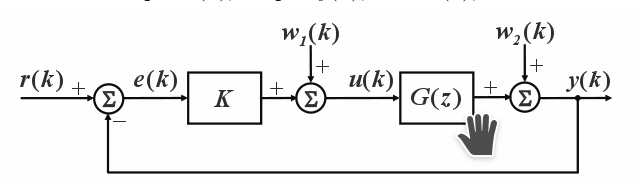
\includegraphics[width=0.5\textwidth]{PR_2_diagram.png}
    \caption{A block diagram for this problem's system}
\end{figure}
The sample period $T=0.5$ seconds, and $G(z)$ is known to have one pole outside the unit circle in the z plane. The discrete Bode Plot of $KG(z)$ is shown on the next page for $K=3$. Do the following problems.
\subsection*{(a)}
Sketch the Nyquist plot for this system on the axes provided on page 3. Be sure to indicate the countour (and direction) you are assuming in sketching the Nyquist plot, and be sure to clearly mark all crossings of all axes in your Nyquist plot. Try to make your Nyquist plot reasonably accurate in the critical areas.\\

The drawn nyquist plot can be seen below.
\begin{figure}[H]
    \centering
    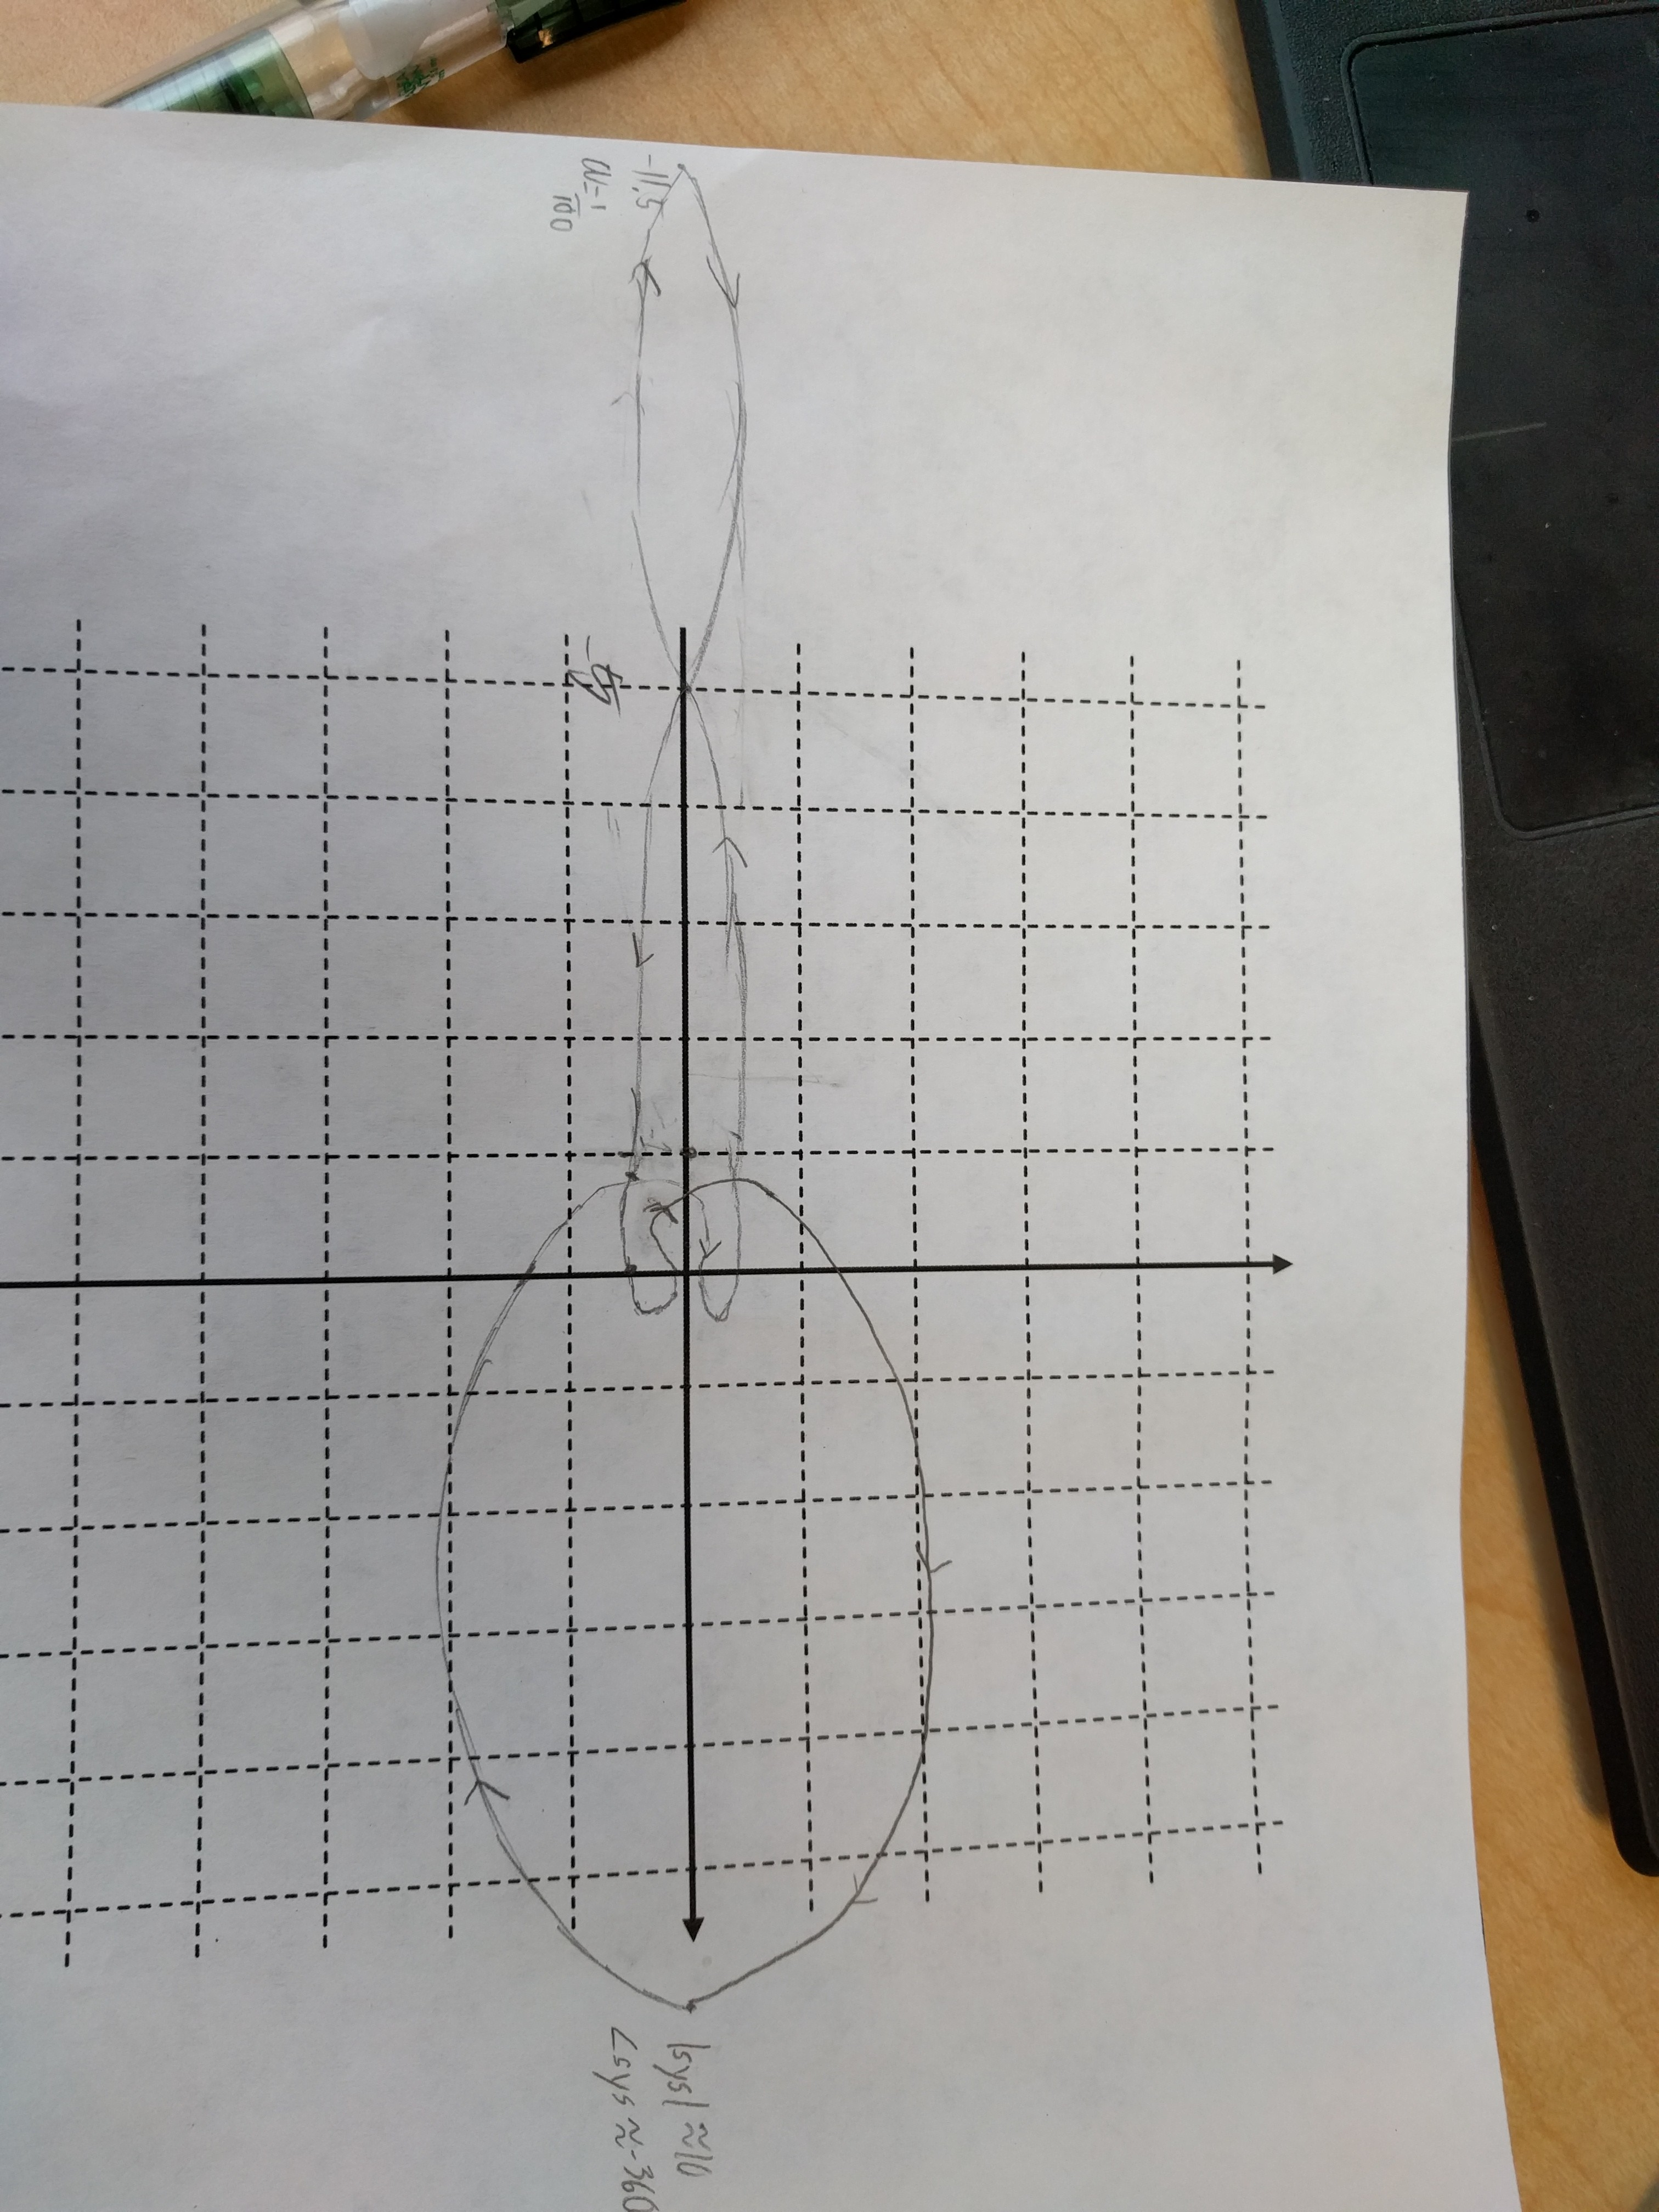
\includegraphics[angle=90,width=0.7\textwidth]{PR2_nyquist.jpg}
    \caption{The nyquist plot for this problem}
\end{figure}
\subsection*{(b)}
For what range(s) of K, both positive and negative, is the system stable? For what range(s) of K, both positive and negative) is the system unstable? How many unstable poles are there in these unstable range(s)? If the number of unstable poles for different ranges changes, list each range separately.\\

Given that the nyquist plot crosses the origin at 5, and there is one counterclockwise encirclement of the origin as well as one pole outside the unit circle, we know that if $K>\frac{3}{5}$ the system will be stable. Otherwise it will be unstable. There is 2 poles outside the origin for the unstable region because there is 1 clockwise encirclement of the origin.
\subsection*{(c)}
For each range of K given in part (b) that leads to a stable closed-loop system, what is the system type with respect to the reference input $r(k)$? What are all range(s) of K such that the closed-loop system is stable and the magnitude of the steady-state error to a unit-step input $r(k)$ is less than $0.1$? Assume $\omega_1(k)$ and $\omega_2(k)$ equal 0.\\

Since the bode plot is not increasing or decreasing at $\omega=0$ the system is type 2 for gains in the stable region of $K>\frac{3}{5}$. Given the equation:
\[K_p>\cfrac{1-e_0}{e_0}=\cfrac{1-0.1}{0.1}=9\]
the gain must be at least 9 to be stable and have a steady state error of less than $0.1$.
\subsection*{(d)}
What are all range(s) of K such that the closed-loop system is stable and the magnitude of the steady-state error to a unit-step distrubance input $\omega_1(k)$ is less than $0.1$? Assume $r(k)=\omega_2(k)=0$.\\

The condition on disturbances between plant and control is that $\lvert D\rvert>>1$ which implies at least one order magnitude bigger than the region for stability. Therefore, $K>35$ will result in a good system.

\subsection*{(e)}
What are all range(s) of K such that the closed-loop system is stable and the magnitude of the steady-state error to a unit-step distrubance input $\omega_2(k)$ is less than $0.1$? Assume $r(k)=\omega_1(k)=0$.\\

One can find the transfer function between $E(z)$ and $W(z)$ to be:
\[\cfrac{E(z)}{W(z)}=\cfrac{-1}{1-KG(z)}\]
So given that $K>3.5$ and the max magnitude of $G(z)=11.5$, we only need that $K>3.5$ for the magnitude of $E(z)$ over $W(z)$ to be less than $0.1$.

\section*{Problem 3}
Given the plant:
\[G(s)=\cfrac{1}{s(s+1)(0.5s+1)}\]
is to be controlled with a digital controller having a sampling period of $T=0.05$ seconds. Answer the following questions. All matlab code is in the appendix.
\subsection*{(a)}
Assuming $G(s)$ is preceded by a ZOH, what is $G(z)$?\\

Using matlab, $G(z)$ was found to be:
\[G(z)=\cfrac{4*10^{-5}(z+3.595)(z+0.258)}{(z-1)(z-0.9512)(z-0.9048)}\]

\subsection*{(b)}
Plot the frequency response (magnitude and phase) of $G(z)$. Using matlab if you want.\\

I used matlabs c2d to get the transfer function here. Then I used the margin command to get the following plot:
\begin{figure}[H]
    \centering
    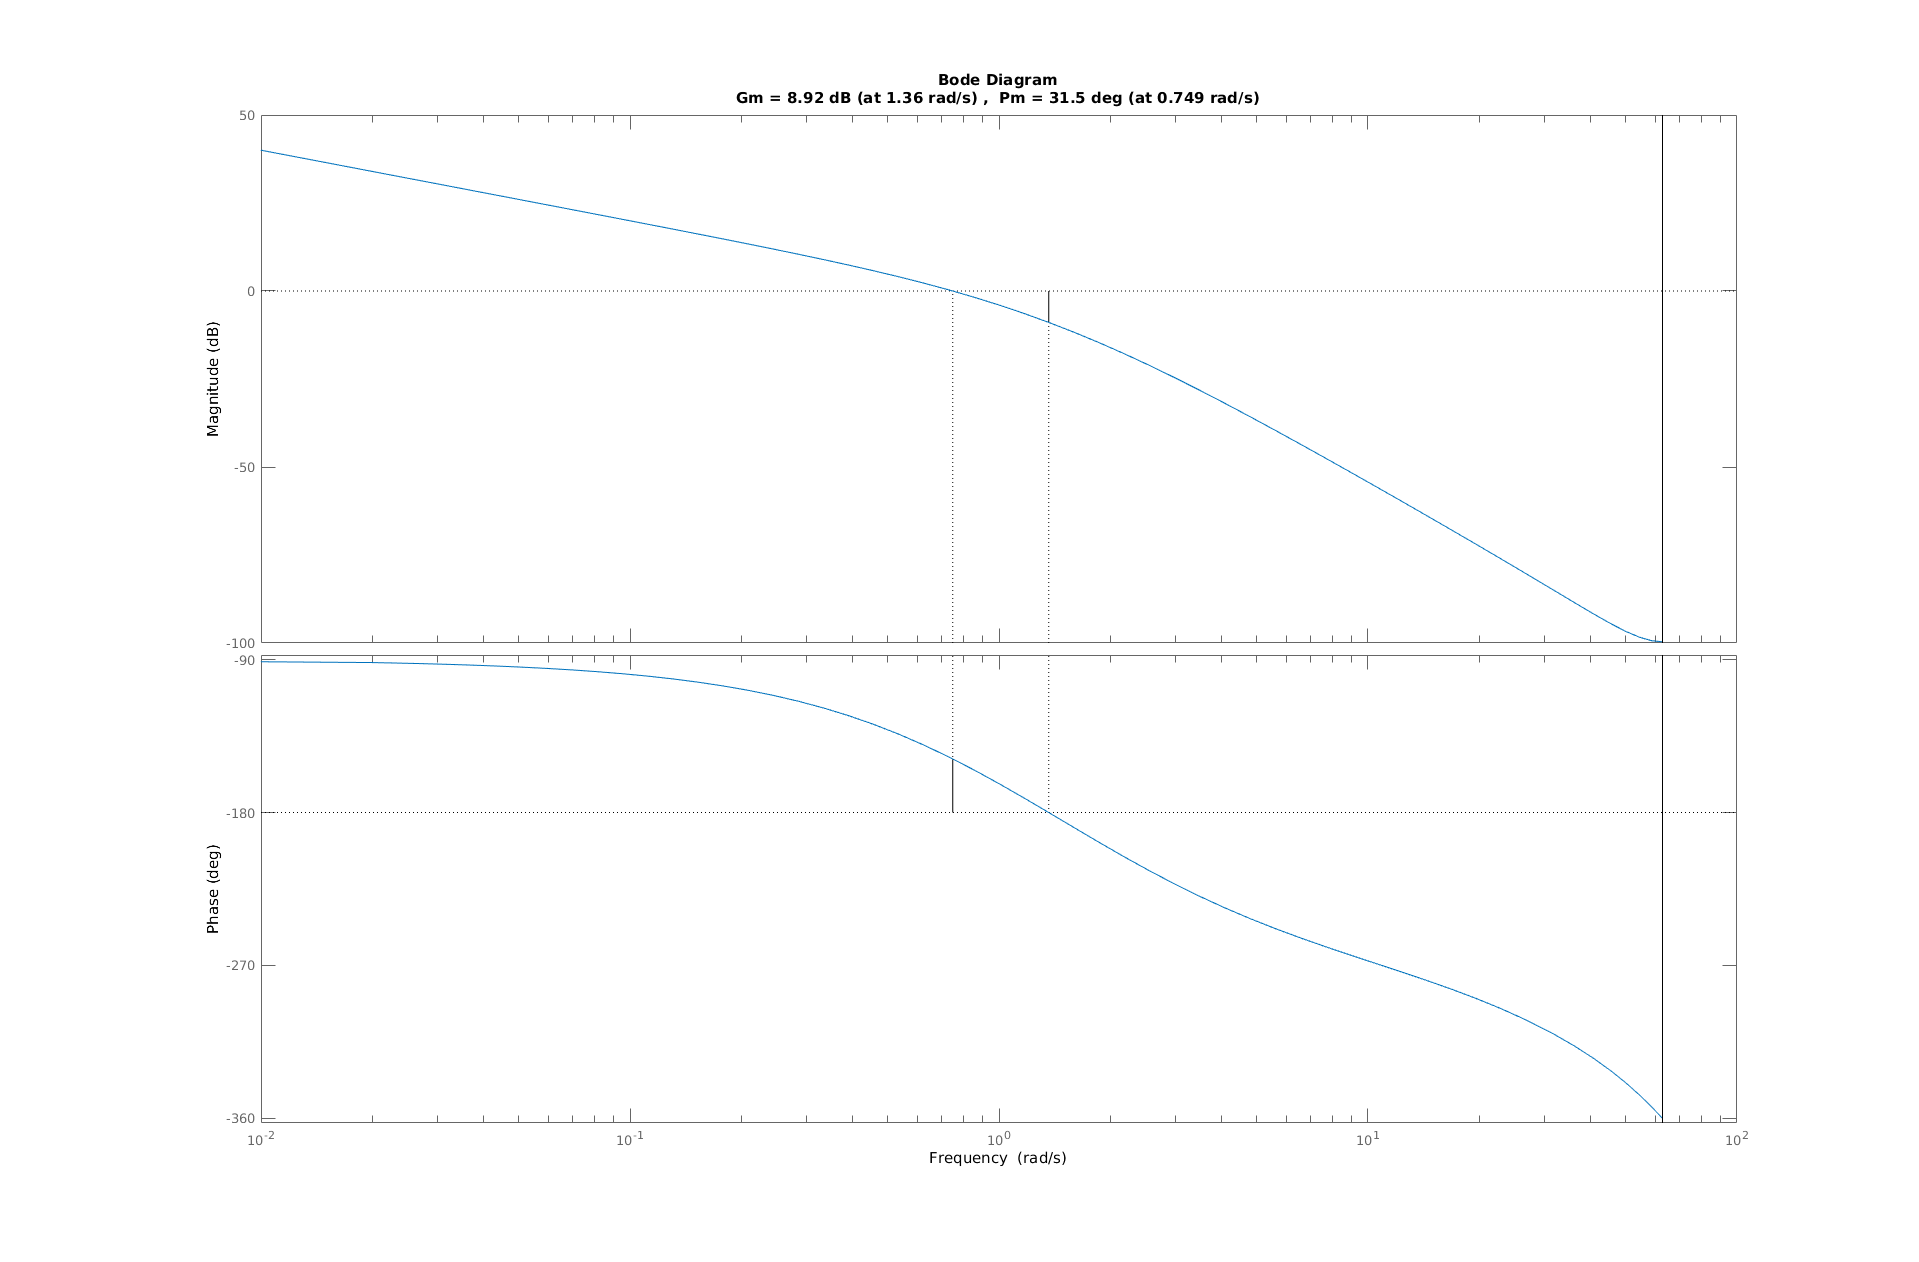
\includegraphics[width=0.8\textwidth]{PR3_bode.png}
    \caption{bode plot with gain and phase margins marked}
\end{figure}
\subsection*{(c)}
Based on the frequency response, what are the gain and phase margins (assuming negative unity feedback)?\\

These are shown in the diagram above. The gain margin is 8.92 dB at 1.36 radians per second. The phase margin is 31.5 degrees at 0.749 radians per second.
\subsection*{(d)}
Sketch the Nyquist plot to double cheeck that the closed-loop system is stable. With $D(z)=K$ preceding $G(z)$ in the closed loop systems forward path. Is there a range of values of $K$ such that the closed-loop system is unstable?\\

I used the nyquist command to plot the nyquist diagram of this system.
\begin{figure}[H]
    \centering
    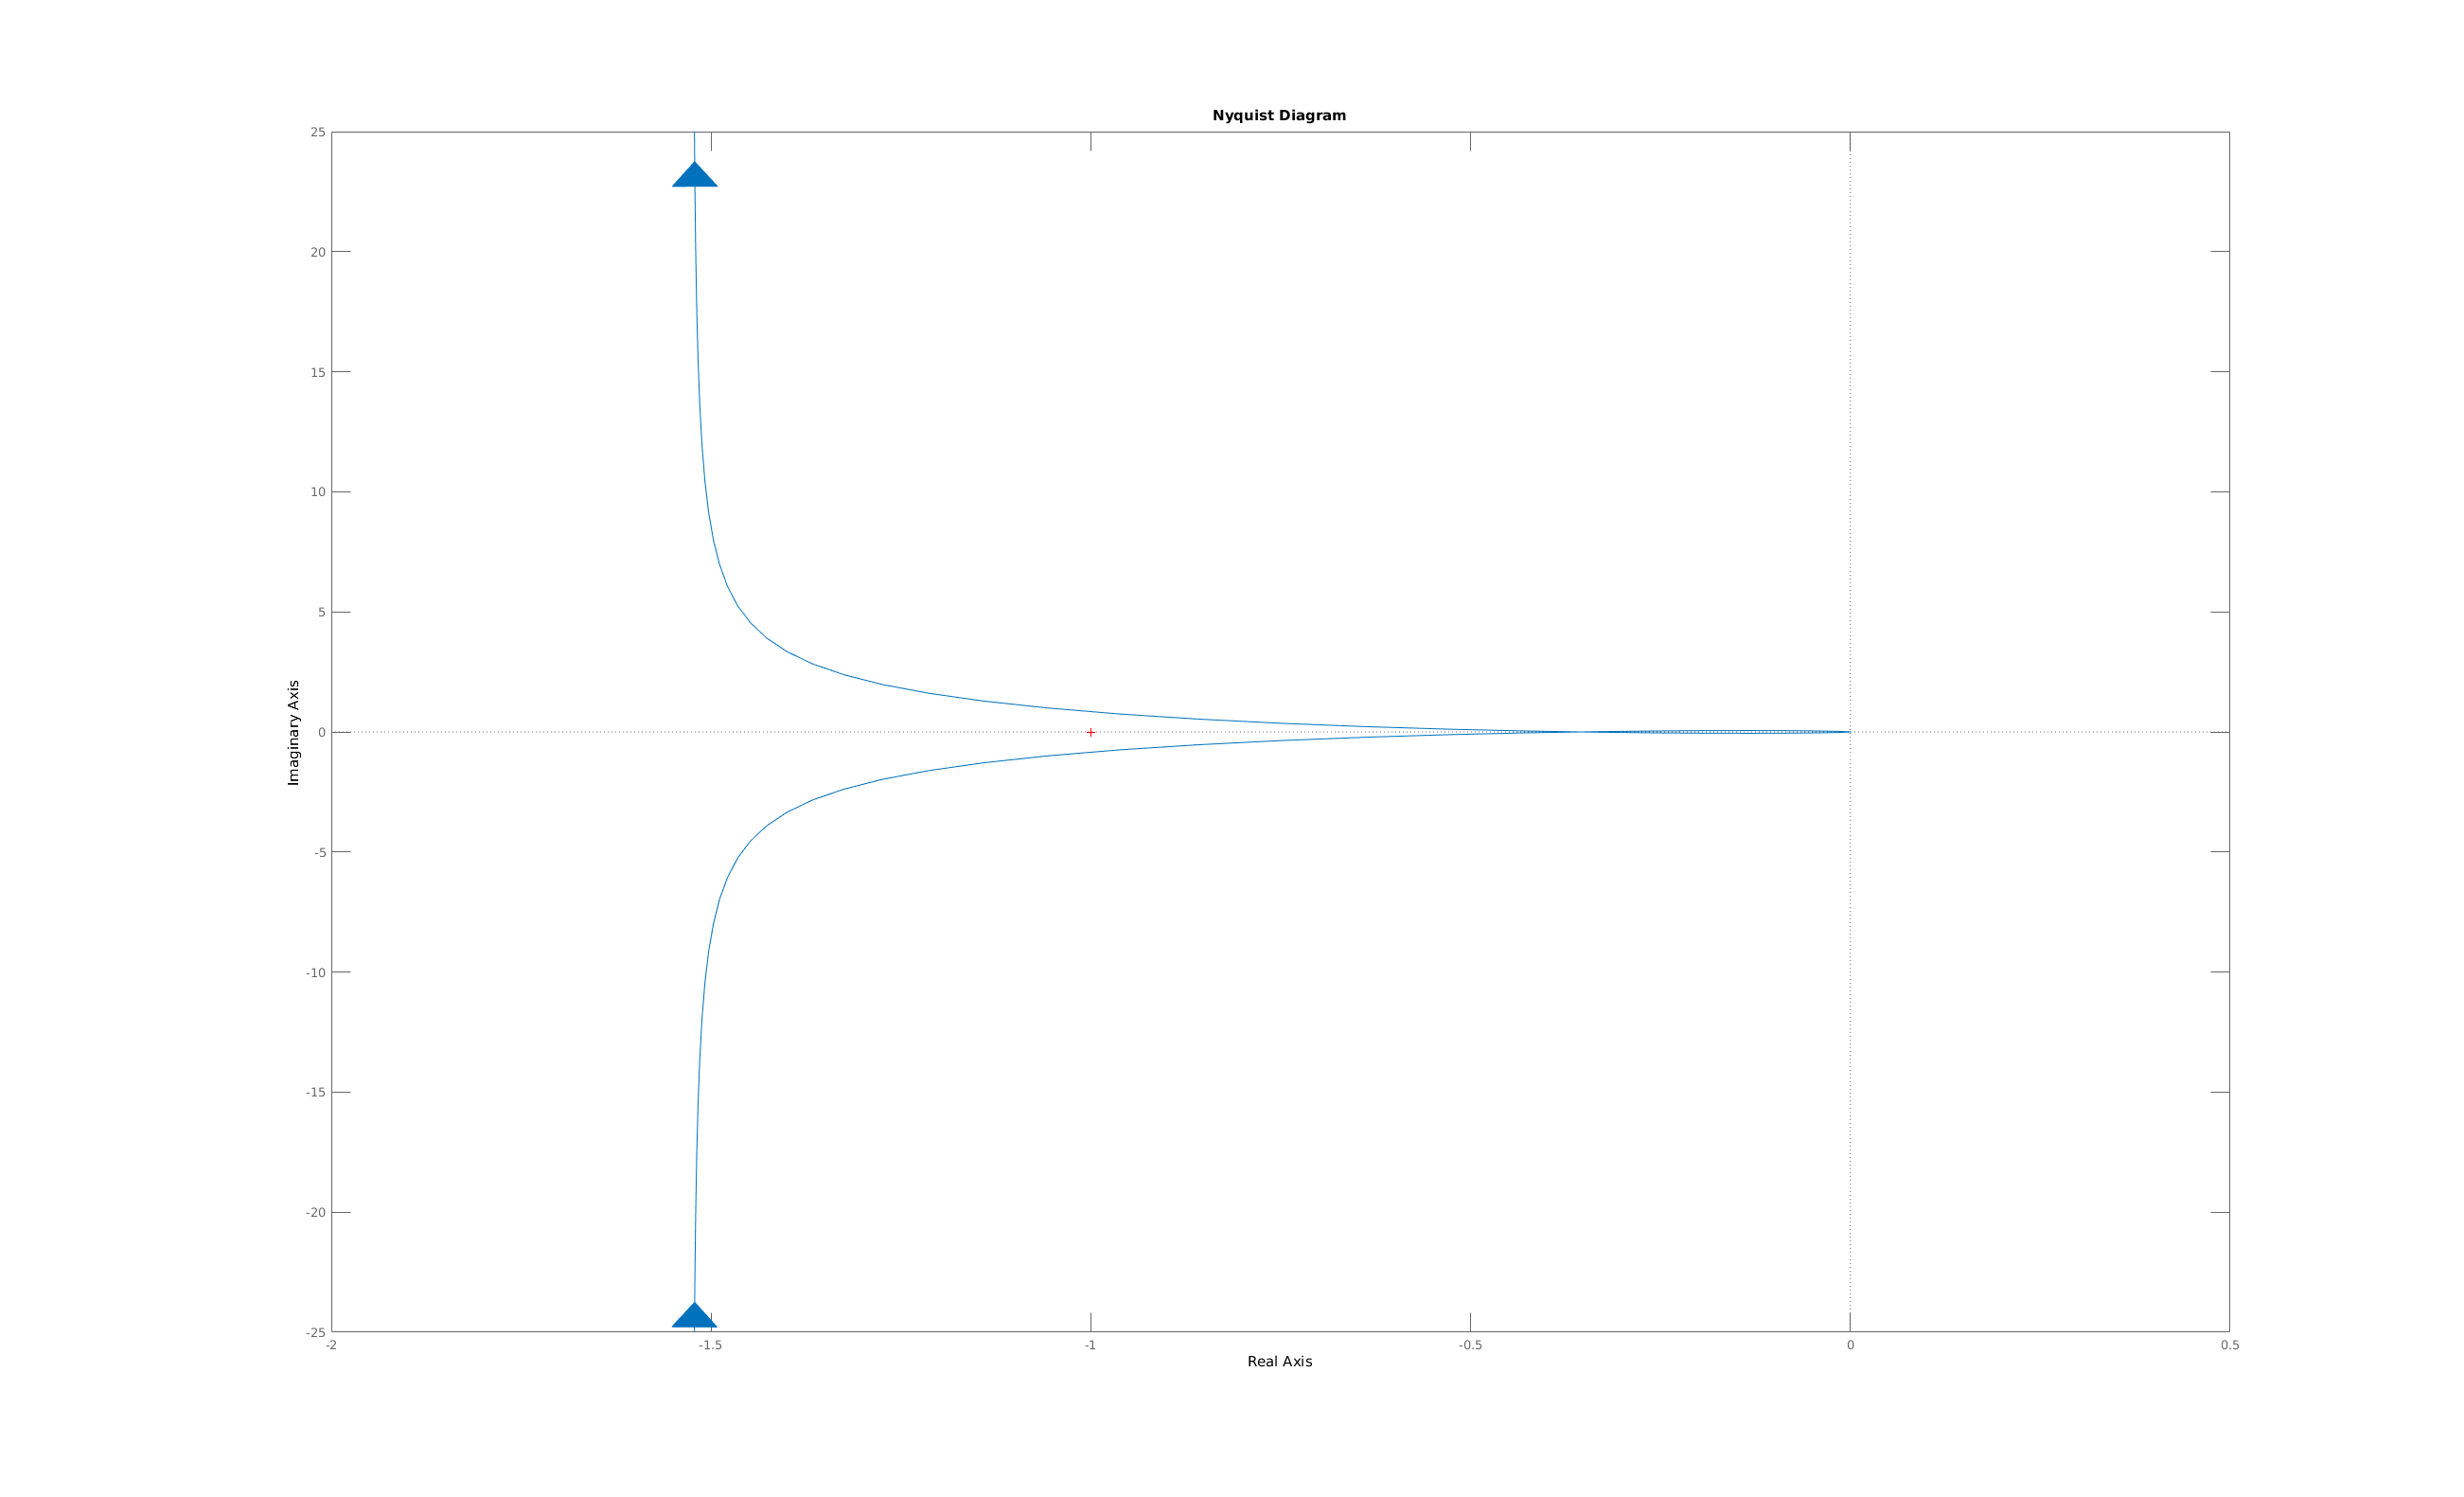
\includegraphics[width=0.8\textwidth]{PR3_nyquist.png}
    \caption{A nyquist plot for the system}
\end{figure}
To determine the $K$ value that leads to an unstable system I found when the data from the nyquist plot passed the axis. Then I took the two values closest to this point, and averaged their magnitudes. The recipricol of this magnitude was the gain needed to make the system unstable and is around $K=2.558$.

\subsection*{(e)}
Design a lag compensator of the form:
\[G(z)=K\cfrac{z+z_1}{z+p_1}\]
so that the phase margin is more than $45^\circ$ and the steady-state error of the closed-loop system to a "unit" ramp input is less than $0.2$.\\

First, we know that $\omega_z T=1-z_1$ and that $\omega_p T=1-p_1$ where $\omega_z=0.2\omega_c=0.1498$rad/sec and $\omega_p=0.02\omega_c=0.01498$rad/sec. Since $T=0.05$ we find:
\[z_1=1-0.1498*0.05=0.9925 \quad p_1=1-0.01498*0.05=0.9993\]
Then we take the limit:
\[\lim_{z=1}\cfrac{K_d(z-0.9925)}{z-0.9993}=0.2\]
This gives $K_d=0.0933$. The phase margin for this is 176 degrees. That technically satisfies the specification so we are done


\section*{Problem 4}
Consider the plant:
\[G(z)=\cfrac{z+3}{z+2}\]
in the standard closed-loop error feedback configuration. Here we will use the Ragazzini direct design method to determine compensator $D(z)$ that stabilize the system. Let $H(z)$ denote the overall closed-loop transfer function from $r(k)$ to $y(k)$. Solve the following problems.
\subsection*{(a)}
What is the minimum relative degree allowed for $H(z)$? That is, what is the minimum number of zeros at infinity that $H(z)$ must have?\\

The minimum relative degree of $H(z)$ is zero as the relative degree of $G(z)$ is zero.
\subsection*{(b)}
What constraints must $H(z)$ satisfy such that the closed-loop system is stable? In other words, what poles and/or zeros of $G(z)$ are not allowed to be canceled by $D(z)$, and what constraints do these yield for $H(z)$?\\

Here, we see that $1-H(z)=(z+2)*()$. This implies that $H(-2)=1$. Similarly, $H(z)=(z+3)*()$, which implies that $H(-3)=0$.
\subsection*{(c)}
Is it possible to have a stable first-order closed-loop $H(z)$ of the following form:
\[H(z)=K\cfrac{z-z_1}{z-p_1}\]
for a real and positive scalar gain $K>0$, and a real zero and pole $z_1,p_1$? If so, determine particular values of $K>0$, $z_1$, and $p_1$ that are feasible and calculate the particular feedback compensator $D(z)$ that yields this stable first-order $H(z)$. Further, compute the steady-state error $e_{ss}=\lim_{k\to\infty}e(k)$ when the reference input $r(k)$ is a discrete-time unit step input. If it is not possible to achieve the above first-order closed-loop $H(z)$, carefully explain
why not.\\

Given that $H(-3)$ is zero we must have:
\[H(z)=K\cfrac{z+3}{z-p_1}\]
Since we also want the system to be stable, $\lvert p_1\rvert<1$. However, $H(-2)=1$, so
\[1=H(-2)=\cfrac{K}{-2-p_1}\]
Since K is strictly positive, $p_1<-2$, but $\lvert p_1\rvert<1$ for stability, so we have formed a contradiction and this realization is impossible.

\subsection*{(d)}
Is it possible to achieve a stable second-order closed-loop $H(z)$ of the following form:
\[H(z)=K\cfrac{z-z_1}{z(z-p_1)}\]
for a real and positive scalar gain $K>0$, and real poles and zeros $z_1,p_1$? If so, determine particular values of $K>0$, $z_1$, and $p_1$ that are feasible and calculate the particular feedback compensator $D(z)$ that yields this stable first-order $H(z)$. Further, compute the steady-state error $e_{ss}=\lim_{k\to\infty}e(k)$ when the reference input $r(k)$ is a discrete-time unit step input. If it is not possible to achieve the above first-order closed-loop $H(z)$, carefully explain why
not.\\

We have the same constraints as the last problem so $H(z)$ is of the form:
\[H(z)=K\cfrac{z+3}{z(z-p_1)}\]
Now we need $K>1$, $\lvert p_1\rvert<1$ and $H(-2)=1$. This gives:
\[1=H(-2)=\cfrac{K}{4+2p_1}\]
Picking $p_1=0.5$ gives $K=5$ and the transfer function is:
\[H(z)=5\cfrac{z+3}{z(z-0.5)}\]
Plotting its step and impulse response gives:
\begin{figure}[H]
    \centering
    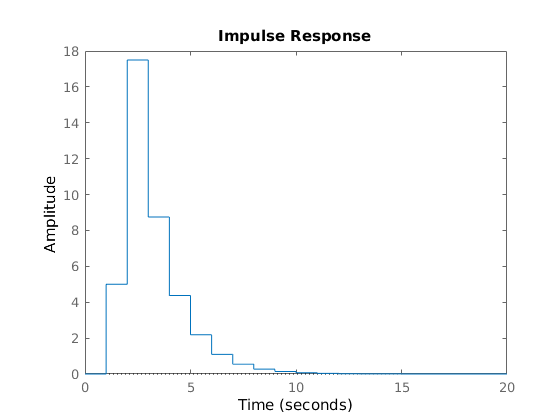
\includegraphics[width=0.7\textwidth]{PR4_impulse.png}
    \caption{impulse response of our system}
\end{figure}
\begin{figure}[H]
    \centering
    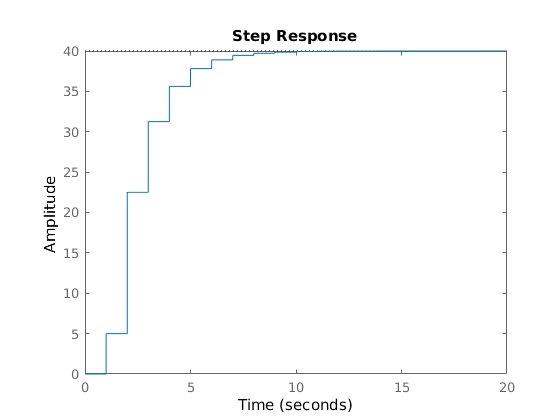
\includegraphics[width=0.7\textwidth]{PR4_step.png}
    \caption{step response of our system}
\end{figure}
The controller is:
\[D(z)=\cfrac{5(z+2)}{z^2-5.5z-15}\]
Given a step input, the steady state value is:
\[e_{ss}=\lim_{z\to1}(z-1)(1-H(z))R(z)=\cfrac{z(z-.5)}{z-.5}-\cfrac{5(z+3)}{z-.5}=-39\]
Thus the steady state error is -39.
\section*{Problem 5}
Use Ragazzini's direct design method to find a compensator $D(z)$ for the transfer function:
\[G(z)=\cfrac{T^2}{2}\cfrac{z+1}{(z-1)^2}\]
corresponding to a ZOH and the continuous $G(s)=\frac{1}{s^2}$ often found in mechanical systems at low frequencies. Here $T=1$ second such that all the closed-loop poles are at $z=0$ (Assume as we have been doing in class that $D(z)$ and $G(z)$ are in the forward path of a negative unity-feedback system). Why would placing all the closed-loop poles at $z=0$ be desirable? Sketch the locus of closed-loop poles as a function of the gain in the resulting compensator $D(z)$. Further, sketch
the step response of the closed-loop system for the particular chosen gain in $D(z)$ from the direct design method.\\

We find $H(z)$ to be:
\[H(z)=\cfrac{1}{2}\cfrac{z+1}{z^2}\]
with the constraints $H(-1)=0$ and $H(1)=1$. Having the poles at the origin gives the system the ability to track any step input accurately. The locus of the system is found by finding $1-H(z)$ and plotting its locus. This was done in Matlab and can be seen below. The step response is also shown below. The code can be found in the appendix.
\begin{figure}[H]
    \centering
    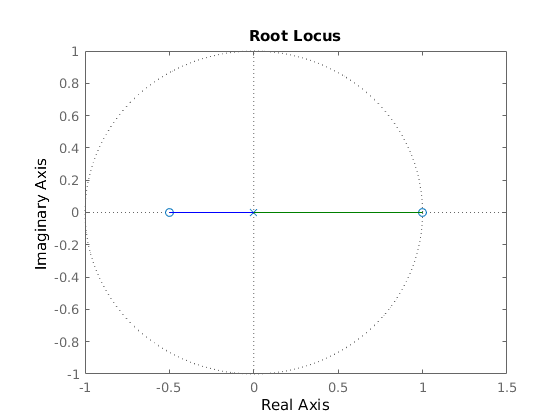
\includegraphics[width=0.7\textwidth]{PR5_locus.png}
    \caption{The locus of $1-H(z)$}
\end{figure}
\begin{figure}[H]
    \centering
    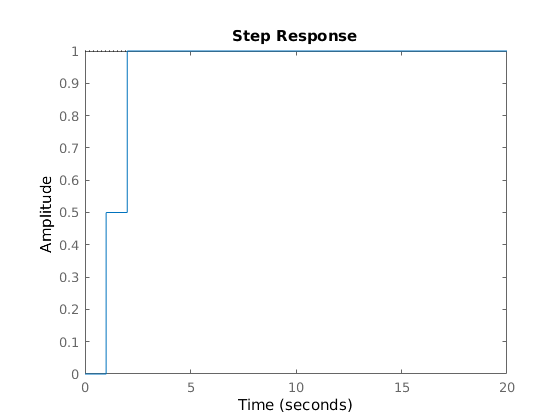
\includegraphics[width=0.7\textwidth]{PR5_step.png}
    \caption{The step response of $H(z)$}
\end{figure}

\appendix
\section*{Appendix}
PR3
\lstinputlisting{PR3.m}
\vspace{1em}
PR4
\lstinputlisting{PR4_test.m}
\vspace{1em}
PR5
\lstinputlisting{PR5.m}
\end{document}
